\documentclass[8pt, a4paper, landscape, includeheadfoot]{extarticle}

% Verwendete Pakete

	\usepackage[utf8]{inputenc}
	\usepackage[top=0.2cm, 
	            bottom=0.01cm, 
	            left=0.5 cm, 
	            right=0.5 cm, 
	            footskip = 2.9pt]{geometry}
	\usepackage{babel} % set language to new german
	\usepackage{amsmath}
	\usepackage{amsfonts}
	\usepackage{lmodern}
	\usepackage{graphicx}
	\setlength{\parindent}{0pt}
	\usepackage{ulem} %option rausgenommen
	\usepackage[dvipsnames]{xcolor}%option "table" raus
	\usepackage{enumitem}
	\usepackage{mathabx}
	\usepackage{enumitem}
	\usepackage{colortbl}
	\usepackage{mathtools}
	\usepackage{wallpaper}
	\usepackage{changepage}
	\usepackage{tikz}
	\usepackage{tabularx}
	\usepackage[skins]{tcolorbox}
	\usepackage{lipsum}
	\usepackage{multicol}
	\usepackage{multirow}
	\usepackage{letltxmacro}
	\usepackage{tabularx}
	\usepackage{float}
    \usepackage{amssymb, physics}
    \usepackage{empheq}
    \usepackage{textcomp} % gensymb dependency
    \usepackage{calc} % Multiplikation mit werten ermöglichen
    \usepackage[makeroom]{cancel} %Terme durchstreichen
    \usepackage{mathtools}
    \usepackage{sidecap} %für Bild und Text nebeneinander
    %\usepackage{gensymb} % Degree celcius symbol
    \usepackage{fancyhdr} % Kopfzeile
    \usepackage{romannum} % roman numbers
	\usepackage{makecell} % zeilenumbruch in tabellen


% Spalteneinstellungen

\setlength\columnsep{5mm}
\setlength{\columnseprule}{0.5pt}

%FBOX Einstellungen

\setlength{\fboxrule}{0.5pt}

%Kopf und Fusszeile 

\setlength{\headsep}{0.5em}
\setlength{\footskip}{2.9pt}

\pagestyle{fancy}
\fancyhf{}
\lhead{\textbf{\Subject}}
\chead{Page \thepage{}}
\rhead{\CustomAuthor}
\cfoot{}

% Farbe

\def \customColor {PineGreen}

% Bullet-Symbol für Aufzählungen
\renewcommand\textbullet{\ensuremath{\bullet}}

% Eingekreiste Nummern für Aufzählungen
\newcommand*\circled[1]{\tikz[baseline=(char.base)]{
        \node[shape=circle,draw,inner sep=1.2pt] (char) {#1};}}

% Schriftart
\renewcommand{\familydefault}{\sfdefault}

%Tabelle Horiz. Grösse
\renewcommand{\arraystretch}{1.5}

%Einheiten
\newcommand{\Einheit}[1]{
$\bigl[ #1 \bigr]$
}

\newcommand{\EinheitBruch}[2]{
$\bigl[ \frac{#1}{#2} \bigr]$
}

\newcommand{\Umbruch}{\vfill\null\columnbreak}

% Titel-Block	
\newcommand{\Header}[3]{
	\begin{tcolorbox}  [arc = 0mm, 
	                    colback = \customColor!50!black, 
	                    colframe = \customColor!50!black, 
	                    valign = center, 
	                    fontupper=\color{white}]
		\large \center \textbf{#1} \par
		\huge \textbf{#2} \par 
		\vskip 5pt 
		\large #3 \par
		\vskip 3pt 
		\small Version: \today
	\end{tcolorbox}
	}

%Teil-Block
\newcommand{\Abschnitt}[1]{
	\begin{tcolorbox} [arc = 0mm,
						colback = \customColor!50!black,
						colframe = \customColor,
						valign = center,
						before skip = 3mm,
						leftright skip = -0.5mm,
						after skip = 1 mm,
						bottomrule = 0 mm,
						toprule = 0 mm,
						leftrule = 0 mm,
						rightrule = 0 mm,
						fontupper=\color{white}
						]
		\centering\Large\textbf{#1}
	\end{tcolorbox}
}

% Überschrift
\renewcommand{\section}[1]{
	\begin{tcolorbox}[
			arc=0mm,
			colback=\customColor!50!black,
			colframe=white,
			bottomrule = 0 mm,
			toprule = 0 mm,
			leftrule = 0 mm,
			rightrule = 0 mm,
			valign=center,
			left=0.5mm,
			top= 0.7 mm,
			bottom= 0.7 mm,
			fontupper=\color{white},
			before skip = 1mm,
			leftright skip = -0.5mm,
			after skip = 1 mm]

		\textbf{#1}
	\end{tcolorbox}
	}

% Abschnitt	
\renewcommand{\subsection}[1]{
\begin{tcolorbox}[
            		arc=0mm,
            		colback=\customColor!50,
            		colframe=white,
            		bottomrule = 0 mm,
            		toprule = 0 mm,
            		leftrule = 0 mm,
            		rightrule = 0 mm,
            		valign=center,
            		left=0.5mm,
            		top=0.2mm,
            		bottom=0.2mm,
            		before skip = 1mm,
            		leftright skip = -0.5mm,
            		after skip = 1mm]
	\small \textbf{#1}
\end{tcolorbox}
}

\renewcommand{\subsubsection}[2]{
\begin{tcolorbox}[
            		arc=0mm,
            		colback=gray!50,
            		colframe=white,
            		bottomrule = 0 mm,
            		toprule = 0 mm,
            		leftrule = 0 mm,
            		rightrule = 0 mm,
            		valign=center,
            		left=0.5mm,
            		top=0.2mm,
            		bottom=0.2mm,
            		before skip = 1mm,
            		leftright skip = -0.5mm,
            		after skip = 1mm]
	\small #1 \hfill #2
\end{tcolorbox}
}

%MATH-BOX, optional commands in {}
\newtcbox{\mathbox}[1][]{%
    nobeforeafter, 
    tcbox raise base, 
    colframe=blue!30!black,
    colback=blue!20, 
    boxrule=1pt,
    arc=1mm,
    before skip = 0mm,
    right = 1mm,
    left=1mm,
	top=0.5mm,
	bottom=0.5mm,
    #1}
    
\newtcbox{\mathboxnoback}[1][]{%
    nobeforeafter, 
    tcbox raise base, 
    colframe=black,
    colback=white,
    boxrule=1pt,
    arc=1mm,
    before skip = 0mm,
    right = 1mm,
    left=1mm,
	top=0.5mm,
	bottom=0.5mm,
    #1}
    
\newcommand{\textbox}[1]{
\tcbox[
		arc=1mm,
		colback=blue!20,
		colframe=blue!30!black,
		arc=1mm,
		boxrule=1pt,
		right = 1mm,
        left=1mm,
	    top=0.5mm,
	    bottom=0.5mm,
		before skip = 1mm,
		after skip = 2 mm
		]
{    
	#1
}
}

\newcommand{\textboxmithead}[2]{
\begin{tcolorbox}[
		arc=1mm,
		colback=blue!20,
		colframe=blue!30!black,
		arc=1mm,
		boxrule=1pt,
		left=1mm,
		top= 1 mm,
		bottom= 1 mm,
		before skip = 2mm,
		leftright skip = 8mm,
		after skip = 2 mm
		]
    \centering{\textbf{#1}\par}
	#2
\end{tcolorbox}
}

\newtcolorbox{titlebox}[1][]{
        fonttitle=\bfseries, 
        colbacktitle=gray!80,
        enhanced,
        attach boxed title to top center={yshift=-2mm},
        colframe=black,
        colback=white,
        boxrule=1pt,
        arc=1mm,
        before skip = 2mm,
        right = 1mm,
        left=1mm,
    	top=0.5mm,
    	bottom=0.5mm,
        title=#1}



\def \Subject {CS229 - Machine Learning}
\def \CustomTitle {Linear Algebra \& Probability}
\def \CustomAuthor {Tim Reinhart - rtim@stanford.edu}

\begin{document}
\pagenumbering{arabic}
\begin{multicols*}{4}
\Header{\Subject}{\CustomTitle}{\CustomAuthor}

\section{Matrices}

\subsection{Matrix Multiplication}

Matrices can be multiplied with each other in the following manner:

\begin{center}
\fbox{
$A \cdot B = C \hspace{5pt} \Rightarrow \hspace{5pt} c_{ik} = \sum_{j=1}^n a_{ij} \cdot b_{jk}$
}
\end{center}

\begin{center}
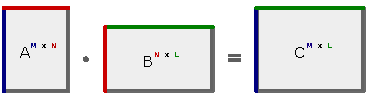
\includegraphics[width = 0.95 \columnwidth]{0_images/Matrixmultiplikation.pdf}
\end{center}

\textbf{Associative \& Distributive Laws:}

\begin{center}
\parskip3pt
\begin{align}
(A\cdot B) \cdot C &= A \cdot (B \cdot C) \nonumber \\
(A + B) \cdot C &= A \cdot C + B \cdot C \nonumber \\
A \cdot (C + D) &= A \cdot C + A \cdot D \nonumber
\end{align}
\end{center}
\textbf{Warning!} The commutative law does not apply! Generally, $A\cdot B \neq B \cdot A$.

\subsection{Transpose}

The transpose of a matrix is obtained by "mirroring" it along its diagonal.

\begin{center}
\textbf{Example:} 
$\begin{pmatrix}
a & b \\
c & d \\
e & f \\
\end{pmatrix}^T
=
\begin{pmatrix}
a & c & e \\
b & d & f \\
\end{pmatrix}$
\end{center}

\textbf{Calculation Rules:}

\vspace{-5mm}
\begin{minipage}[t]{0.49 \columnwidth}
\begin{align}
(A + B)^T &= A^T + B^T \nonumber \\
(A \cdot B)^T &= B^T \cdot A^T \nonumber \\
(c \cdot A)^T &= c \cdot A^T \nonumber \\
(A^T)^T &= A \nonumber
\end{align}
\end{minipage}
\begin{minipage}[t]{0.49 \columnwidth}
\begin{align}
(A^T)^{-1} &= (A^{-1})^T \nonumber \\
rank(A^T) &= rank(A) \nonumber \\
det(A^T) &= det(A) \nonumber \\
eig(A^T) &= eig(A) \nonumber
\end{align}
\end{minipage}


\subsection{Inverse}

The inverse \( A^{-1} \) of \( A \) reverses a multiplication with \( A \). When you multiply \( A \) with \( A^{-1} \), you get the identity matrix.

\textbf{Properties:}

\begin{itemize}[leftmargin=0.29cm, itemsep=0pt]
\item Only square matrices can be invertible.
\item An invertible matrix is called \textbf{regular}, a non-invertible one \textbf{singular}.
\item The inverse is unique.
\item \( A \) is invertible if and only if \( A \) has full rank.
\item \( A \) is invertible if and only if \( A^T \) is invertible.
\item \( A \) is symmetric if and only if \( A^{-1} \) is symmetric.
\item \( A \) is a triangular matrix if and only if \( A^{-1} \) is a triangular matrix.
\item \( A \) is invertible if and only if \( \text{det}(A) \neq 0 \).
\item \( A \) is invertible if and only if no eigenvalue \( \lambda = 0 \).
\item \( A \) and \( B \) are invertible implies \( AB \) is invertible.
\end{itemize}

\textbf{Calculation rules:}

\vspace{-5mm}
\begin{minipage}[t]{0.49 \columnwidth}
\begin{align}
I^{-1} &= I\nonumber \\
(A^{-1})^{-1} &= A \nonumber \\
(A^k)^{-1} &= (A^{-1})^k \nonumber \\
(c\cdot A)^{-1} &= c^{-1} \cdot A^{-1} \nonumber \\
(A\cdot B)^{-1} &= B^{-1} \cdot A^{-1} \nonumber
\end{align}
\end{minipage}
\begin{minipage}[t]{0.49 \columnwidth}
\begin{align}
(A^T)^{-1} &= (A^{-1})^T \nonumber \\
rang(A^{-1}) &= rang(A) \nonumber \\
det(A^{-1}) &= det(A)^{-1} \nonumber \\
eig(A^{-1} &= eig(A)^{-1} \nonumber 
\end{align}
\end{minipage}

\subsection{Eigenvalues and Eigenvectors}

\begin{empheq}[box = \mathboxnoback]{align*}
    \text{Eigenvalues of A: } \det(A - \lambda\cdot I) = 0
\end{empheq}

\textbf{Verify Computation}

\begin{itemize}[leftmargin=0.29cm, itemsep=0.5pt]
\item Trace(A) = \( a_{11} + a_{22} + \dots + a_{nn} = \sum \lambda_i \)
\item det(A) = product of \( \lambda_i \)
\end{itemize}

\textbf{Eigenvectors: } Kernel of the matrix $A - \lambda_i\cdot I$, where \( \lambda_i \) is the eigenvalue corresponding to the eigenvector.

\subsection{Determinant}

\textbf{Block Sentence for Determinant Computation}

\begin{center}
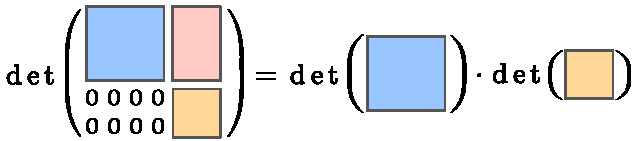
\includegraphics[width = 0.8 \columnwidth]{0_images/Blocksatz.pdf}
\end{center}

\section{Matrix Calculus}

\Umbruch

\section{Probability}
\subsection{Bayes Theorem}

$$
	P( X{=}x  | Y {=} y) = \frac{P(Y{=}y | X{=}x) P(X{=}x)}{P(Y{=}y)}
$$
\subsection{Expectation Value}

\begin{align*}
	\operatorname{E}[X] \,= \sum_i x_i p_i \text{ or } \operatorname{E}[X]\equiv\int_\Omega X\,d\operatorname{P}=\int_{\mathbb{R}}xf(x)\,dx
\end{align*}

\subsubsection{Conditional Expectation}{}
\begin{align*}
	\operatorname{E} (X \mid Y=y) =  \sum_x x P(X = x \mid Y = y) \\
	= \sum_x x \frac{P(X = x, Y = y)}{P(Y=y)}
\end{align*}
\subsection{Variance}
\begin{align*}
	Var(X) = \operatorname{E}[\left(X-\mu\right)^2] = \operatorname{E}[X^2] - \operatorname{E}[X]^2
\end{align*}
\subsection{Exponential Family}
A single-parameter exponential family is a set of probability distributions 
whose probability density function (or probability mass function, for the case of a discrete distribution) can be expressed in the form
$$
p(y;\eta) = b(\eta)\,\exp\bigl[\,\eta^T \, T(y) - a(\eta)\,\bigr]
$$
\begin{itemize}[itemsep=0pt]
	\item $\eta$: natural parameter
	\item $T(y)$: sufficient statistic
	\item $a(\eta)$: log partition function
\end{itemize}

\subsubsection{Canonical Response Funtion}{}
$$
g(\eta) = \operatorname{E}[T(y);\eta]
$$
\begin{itemize}[itemsep=0pt]
	\item For the Gaussian family: identify function
	\item For the Bernoulli family: logistic function
\end{itemize}

\end{multicols*}
\end{document}
